\section{Bootstrapping and results}

\subsection{Energy spectrum}
\autoref{fig:bootstrap:distributions}.

\todo{
  This is (probably) the most important plot. Discuss it in more detail!
  Also: Explain percentiles etc.
}
\blindtext[2]

\begin{figure}
  \centering
  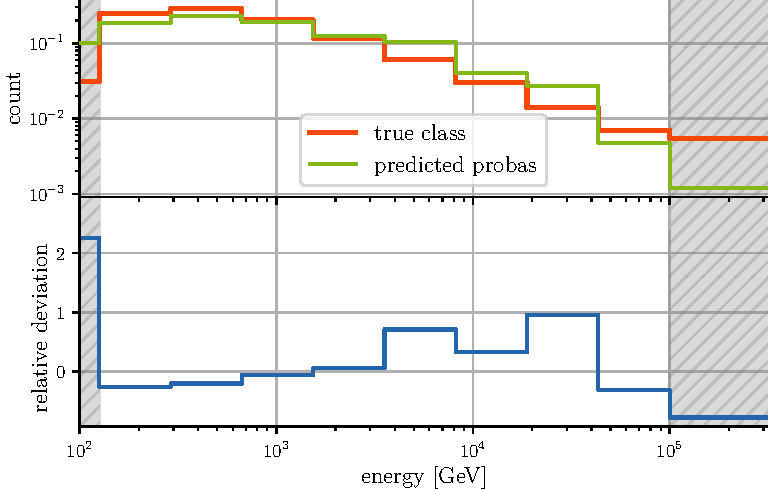
\includegraphics[scale=1]{content/plots/bootstrap:spectrum.pdf}
  \caption{
    Energy spectrum and relative deviations of the bootstrap.
    TODO: Placeholder data.
    % TODO: Add axspan to legend or explain it here.
  }
  \label{fig:bootstrap:spectrum}
\end{figure}


\subsection{Individual events}
Ordinal classification methods promise physically plausible results… % TODO
In contrast to \emph{LogisticAT},
  the unimodality of the probability distribution is not enforced directly.
Instead,
  only the threshold probabilities ($f_k(\mathbf{x}^{[i]})$) are constrained to be monotonically increasing
  by the chain rule of probability
  (see \autoref{sec:corn:method}).
% This means that the probability distribution can be multimodal.
As can be seen in \autoref{fig:bootstrap:single_events},
  slight deviations from unimodality do occur.
  % TODO: Compare to a Random Forest?


\begin{figure}
  \centering
  % TODO: correct dimensions
  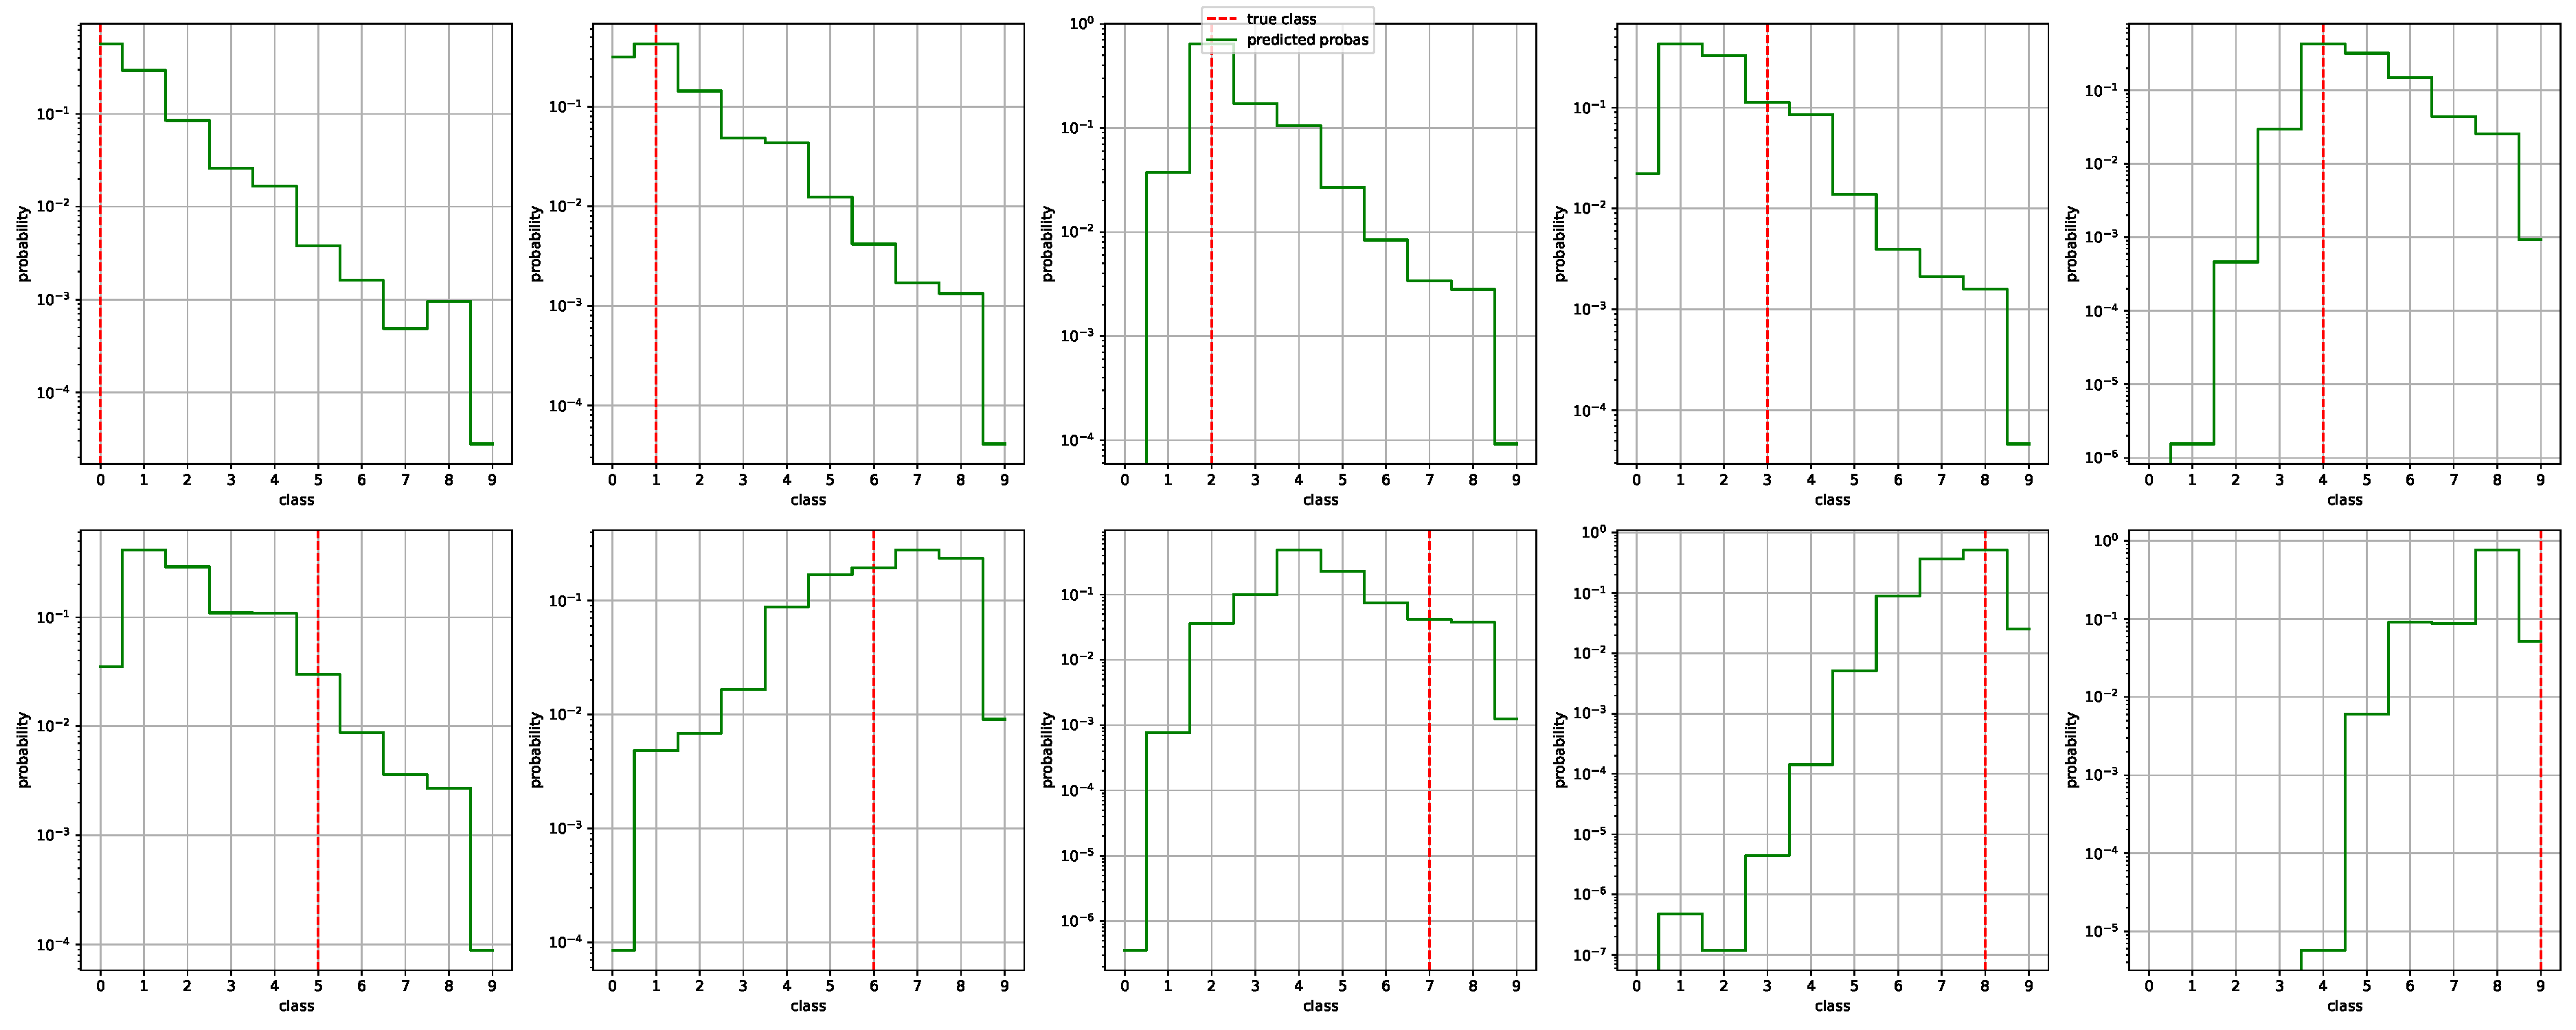
\includegraphics[width=\textwidth]{content/plots/halftime/single_events.pdf}
  \caption{
    Confidence distributions of individual events.
    For each true class,
    one random event is selected from the test set,
    and the confidence distribution of the model is shown.
  }
  \label{fig:bootstrap:single_events}
\end{figure}
